\section{Results and Analysis}\label{sec:simulations}
The specified specifications are verified by the use of simulations. While providing a one tone signal, a transient measurement of the output power is simulated. This to verify a correct functioning DAC, that translates the digitals signals as supposed. This holds that the 15 bit digital unary code is translated to an analogue signal with 16 level resolution.

\begin{figure}[htp] 
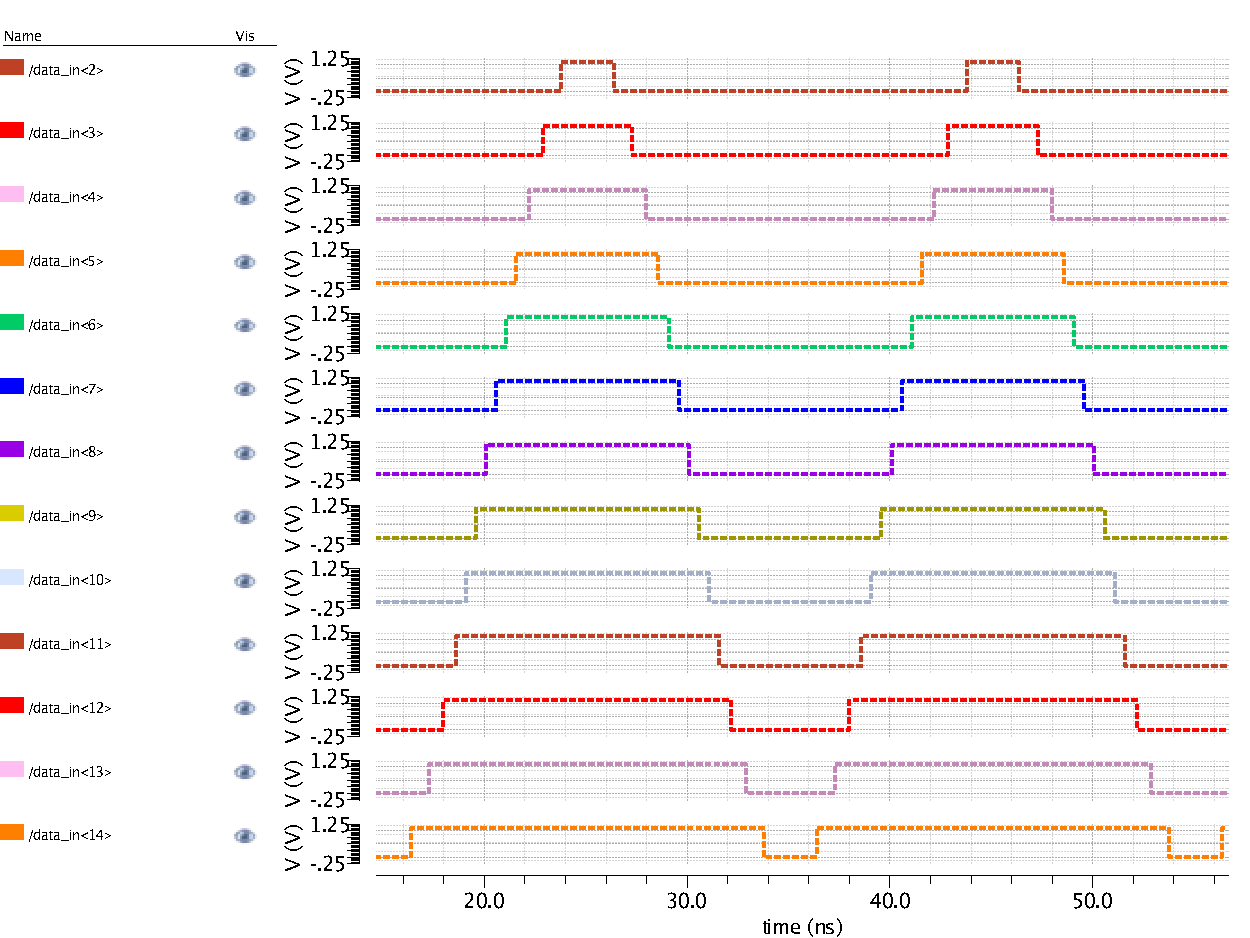
\includegraphics[width=0.5\textwidth]{thermometer_output.pdf}
\caption{Thermometer single tone voltage output.}
\label{fig:Thermometer}
\end{figure}

\begin{figure}[htp] 
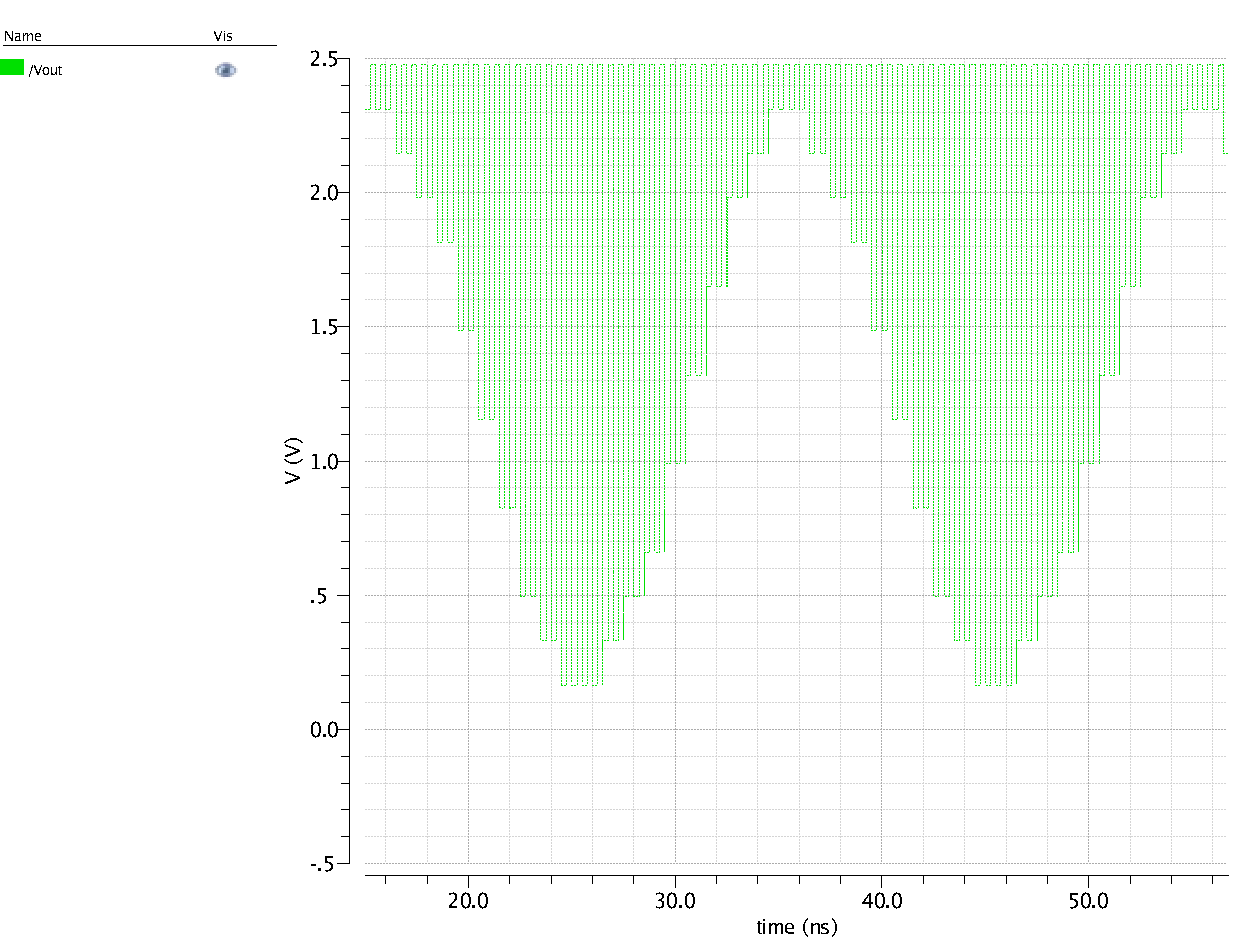
\includegraphics[width=0.5\textwidth]{Vout_ideal.pdf}
\caption{SoC voltage output.}
\label{fig:SoC Vout}
\end{figure}


Next a DFT of the output voltage is simulated to see the spectral content of the one tone model. This to find the power of the harmonic distortion and the spurious-free dynamic range (SFDR).  The SFDR describes the power of the fundamental signal to the strongest spurious signal at the output, which is most commonly the second harmonic. 
Furthermore a two tone test is simulated, the two tone test is useful test the linearity of the DAC. Non-linear behaviour generates intermodulation products at the output of the DAC. The power of these intermodulation products will examined, especially the third intermodulation product (IM3). Because the IM3 frequencies are very close to the fundamental frequency (at 2f2-f1 and 2f1-f2), it is almost impossible to filter it out of the output signal; therefore, it is better to prevent creating them. 